% !TeX program = pdflatex
% Standalone source. Compile with pdfLaTeX; no external figures are required.
\documentclass[11pt,a4paper]{article}
\usepackage[margin=20mm]{geometry}
\usepackage[T1]{fontenc}
\usepackage{lmodern}
\usepackage{amsmath,amssymb,booktabs,array,xcolor,tikz,fancyhdr,hyperref,listings,pgfplots}
\usetikzlibrary{calc,arrows.meta}
\hypersetup{colorlinks=true,linkcolor=blue!50!black,urlcolor=blue!50!black}
\definecolor{accent}{HTML}{124E66}
\definecolor{pcol}{HTML}{A24021}
\definecolor{ncol}{HTML}{175A86}
\pagestyle{fancy}\fancyhf{}\fancyhead[L]{\small EE3032 / Fall 2021 / HW1}
\fancyhead[R]{\small CMOS logic}\fancyfoot[C]{\thepage}
\setlength{\headheight}{15pt}\setlength{\parindent}{0pt}\setlength{\parskip}{6pt}
\renewcommand{\arraystretch}{1.2}
\newcommand{\answer}[1]{\par\noindent\colorbox{accent!9}{\parbox{0.96\linewidth}{#1}}\par}
\newcommand{\AND}{\,}
\newcommand{\VDD}{V_{\mathrm{DD}}}
\newcommand{\VSS}{V_{\mathrm{SS}}}
% A conventional switch-level MOS symbol: continuous channel, insulated gate,
% and a gate bubble for pMOS. Bulk terminals are omitted, as explained below.
% Arguments: device id, x, y, gate literal, p or n. t/b are upper/lower terminals.
\newcommand{\MOS}[5]{
  \coordinate (#1) at (#2,#3);
  \coordinate (#1t) at ($(#1)+(0,.55)$);
  \coordinate (#1b) at ($(#1)+(0,-.55)$);
  \draw (#1t)--($(#1)+(0,.30)$)--($(#1)+(-.18,.30)$);
  \draw ($(#1)+(-.18,.34)$)--($(#1)+(-.18,-.34)$);
  \draw ($(#1)+(-.18,-.30)$)--($(#1)+(0,-.30)$)--(#1b);
  \draw ($(#1)+(-.35,.33)$)--($(#1)+(-.35,-.33)$);
  \def\type{#5}\def\ptype{p}
  \ifx\type\ptype
    \draw ($(#1)+(-.78,0)$)--($(#1)+(-.53,0)$);
    \draw ($(#1)+(-.465,0)$) circle (.065);
    \draw ($(#1)+(-.40,0)$)--($(#1)+(-.35,0)$);
  \else
    \draw ($(#1)+(-.78,0)$)--($(#1)+(-.35,0)$);
  \fi
  \node[anchor=east] at ($(#1)+(-.82,0)$) {$#4$};
  \node[anchor=west,font=\scriptsize] at ($(#1)+(.10,0)$) {#1};
}
% A transmission-gate instance; its two MOS devices are expanded on page 3.
\newcommand{\TG}[4]{
  \node[draw,rounded corners=1pt,minimum width=11mm,minimum height=6mm,
        fill=accent!5,font=\small] (#1) at (#2,#3) {$\mathrm{TG}_{#4}$};
}

\pgfplotsset{compat=1.18}
\lstset{basicstyle=\ttfamily\scriptsize,breaklines=true,frame=single,columns=fullflexible}
\begin{document}
\begin{center}{\LARGE\bfseries 2021 HW1}\\[4pt]{\large MOS Theory, Multiplexers, and Static CMOS}\\[4pt]{\small EE3032 / Introduction to VLSI Design}\end{center}
\textbf{Provenance.} The original assignment and the supplied answers by Lin Yan-Yu were read first. The results below were independently derived, with the useful reference choices retained and improvements identified. Source details and hashes are in the year-level \texttt{SOURCES.md}.

\textbf{Notation.} $+$ is OR; juxtaposition is AND. Every pMOS body is tied to $\VDD$ and every nMOS body to ground. Body terminals are omitted in the diagrams. Only true input literals are used in the CMOS gates below.
\section*{1. Two identical series devices per inverter branch}
\textbf{(a) The rail-side devices $M_1$ and $M_4$ cannot carry nonzero DC current in saturation.}
For the nMOS stack let the internal node be $u$ and $U=V_{\rm in}-V_{tn}>0$.
Saturation of the lower $M_1$ would require $u\ge U$. But then the upper device has
$V_{GS,2}=V_{\rm in}-u\le V_{tn}$ and is cut off. Thus the assumed positive stack current is impossible. The pMOS argument is identical with voltages measured downward from $\VDD$: saturation of rail-side $M_4$ would cut off $M_3$.
At cutoff or the zero-current boundary, the usual region inequalities may coincide; the statement concerns conducting operation.
\textbf{(b) Both equivalent aspect ratios are one half of the original:}
\[
 \boxed{(W/L)_{N_1}=(W/L)_{N_2}=\tfrac12(W/L).}
\]
Here $N_1$ is nMOS and $N_2$ is pMOS. This equality uses the ideal long-channel square-law model, no body effect, and no channel-length modulation; it does not assert exact BSIM short-channel equivalence.
Let $k_n=\mu_n C_{\rm ox}(W/L)$. If the upper nMOS is saturated,
\[
 k_n(Uu-u^2/2)=\frac{k_n}{2}(U-u)^2,
 \quad u=U\left(1-\frac1{\sqrt2}\right),
 \quad I=\frac{k_nU^2}{4}.
\]
A single saturated nMOS with $k_{\rm eq}=k_n/2$ has the same current. If both devices are linear and $v=V_{\rm out}<U$, adding their equal-current equations gives
\[
 \frac{2I}{k_n}=Uv-\frac{v^2}{2},\qquad
 I=\frac{k_n}{2}\left(Uv-\frac{v^2}{2}\right).
\]
Thus the half-aspect-ratio device also matches the linear part of the branch characteristic; the pMOS derivation is symmetric. Halve $W$ at fixed $L$, or double $L$ in this ideal model.
\textbf{Reference comparison.} The supplied answer identifies $M_1,M_4$ and the factor $1/2$ correctly. The present proof also covers the linear region. \texttt{verify\_logic.py} checks 5,050 normalized operating points; the maximum current-equation error is below $10^{-12}$.
\newpage
\section*{2. Exactly two of three inputs are one}
The requested function is
\[
 f=\bar x_1x_2x_3+x_1\bar x_2x_3+x_1x_2\bar x_3
   =\bar x_1(x_2x_3)+x_1(x_2\oplus x_3).
\]
Write $M(s,d_0,d_1)=\bar s d_0+s d_1$. An implementation using four 2:1 multiplexers and constants only is
\[
 n=M(x_3,1,0),\quad g=M(x_2,0,x_3),\quad
 h=M(x_2,x_3,n),\quad \boxed{f=M(x_1,g,h).}
\]
The first mux makes $\bar x_3$ without an inverter; $g=x_2x_3$ and $h=x_2\oplus x_3$.
\begin{center}
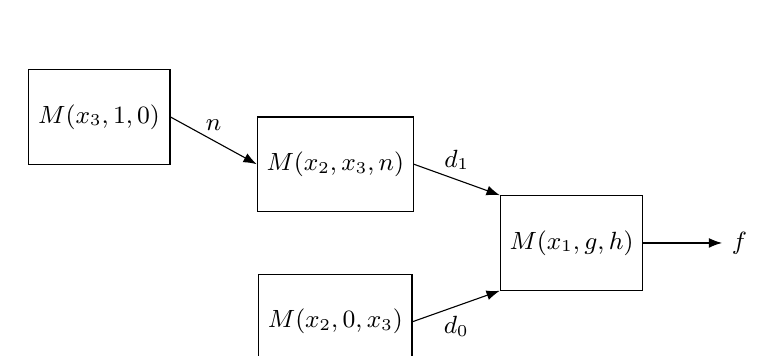
\begin{tikzpicture}[font=\small,>=Latex]
\node[draw,minimum width=18mm,minimum height=12mm] (n) at (0,2.6) {$M(x_3,1,0)$};
\node[draw,minimum width=18mm,minimum height=12mm] (h) at (3,2) {$M(x_2,x_3,n)$};
\node[draw,minimum width=18mm,minimum height=12mm] (g) at (3,0) {$M(x_2,0,x_3)$};
\node[draw,minimum width=18mm,minimum height=12mm] (f) at (6,1) {$M(x_1,g,h)$};
\draw[->] (n.east)--(h.west) node[midway,above] {$n$};
\draw[->] (h.east)--(f.north west) node[midway,above] {$d_1$};
\draw[->] (g.east)--(f.south west) node[midway,below] {$d_0$};
\draw[->] (f.east)--++(1,0) node[right] {$f$};
\end{tikzpicture}
\end{center}
\begin{center}\begin{tabular}{ccc|c}\toprule
$x_1$&$x_2$&$x_3$&$f$\\\midrule
0&0&0&0\\0&0&1&0\\0&1&0&0\\0&1&1&1\\
1&0&0&0\\1&0&1&1\\1&1&0&1\\1&1&1&0\\\bottomrule
\end{tabular}\end{center}
\textbf{Reference comparison.} The supplied full Shannon tree has seven muxes, including constant-only leaves. Its truth table is correct. The factored four-mux circuit saves three muxes while still using muxes exclusively. Exhaustive evaluation of all eight inputs confirms equality.
\newpage
\section*{3(a). Complemented AOI function}
\textbf{Read the overbar in the prompt carefully: it spans the entire sum.}
\[
 \boxed{f(w,x,y,z)=\overline{w(x+y)+yz}.}
\]
The pull-down network (PDN) implements $G=w(x+y)+yz$: $n_w$ in series with $(n_x\parallel n_y)$, in parallel with $(n_y\hbox{ series }n_z)$.
The pull-up network (PUN) is the dual:
$(p_w\parallel(p_x\hbox{ series }p_y))$ in series with $(p_y\parallel p_z)$.
\begin{center}
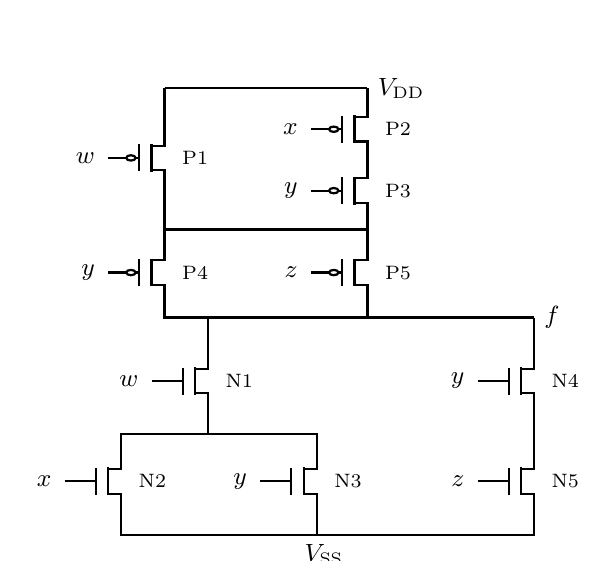
\begin{tikzpicture}[x=.92cm,y=.52cm,line width=.8pt,font=\small]
\MOS{P1}{-.6}{6.1}{w}{p}\MOS{P2}{2.2}{6.8}{x}{p}\MOS{P3}{2.2}{5.3}{y}{p}
\MOS{P4}{-.6}{3.3}{y}{p}\MOS{P5}{2.2}{3.3}{z}{p}
\draw (-.6,7.8)--(2.2,7.8) node[right] {$\VDD$};
\draw (-.6,7.8)--(P1t) (2.2,7.8)--(P2t) (P2b)--(P3t);
\draw (P1b)--(-.6,4.35)--(2.2,4.35)--(P3b);
\draw (-.6,4.35)--(P4t) (2.2,4.35)--(P5t);
\draw (P4b)--(-.6,2.2)--(4.5,2.2) node[right] {$f$};\draw (P5b)--(2.2,2.2);
\MOS{N1}{0}{.65}{w}{n}\MOS{N2}{-1.2}{-1.8}{x}{n}\MOS{N3}{1.5}{-1.8}{y}{n}
\MOS{N4}{4.5}{.65}{y}{n}\MOS{N5}{4.5}{-1.8}{z}{n}
\draw (0,2.2)--(N1t) (4.5,2.2)--(N4t);
\draw (N1b)--(0,-.65)--(-1.2,-.65)--(N2t);\draw (0,-.65)--(1.5,-.65)--(N3t);
\draw (N4b)--(N5t);
\draw (N2b)--(-1.2,-3.1)--(4.5,-3.1)--(N5b);\draw (N3b)--(1.5,-3.1);
\node[below] at (1.6,-3.1) {$\VSS$};
\end{tikzpicture}
\end{center}
There are five nMOS and five pMOS devices: \textbf{10 transistors total}. Two devices are separately controlled by $y$ in each network; they are distinct transistors.
\[
 PUN=\bigl[\bar w+\bar x\bar y\bigr](\bar y+\bar z)
     =\overline{w(x+y)+yz}=f.
\]
Every input has exactly one conducting rail network in ideal switch logic, so there is no static VDD-to-ground path. No complemented external input is needed.
\textbf{Reference comparison.} The supplied diagram uses the same correct 10-transistor topology. This solution retains it, clarifies the overbar, and checks all 16 input combinations.
\newpage
\section*{3(b). Complement of a three-input majority}
\[
 f=\bar x\bar y+\bar x\bar z+\bar y\bar z
   =\overline{xy+xz+yz}
   =\boxed{\overline{x(y+z)+yz}}.
\]
Use the same network structure as 3(a), now with the first branch $n_x$ in series with $(n_y\parallel n_z)$ and the second branch $n_y$ in series with $n_z$.
\begin{center}
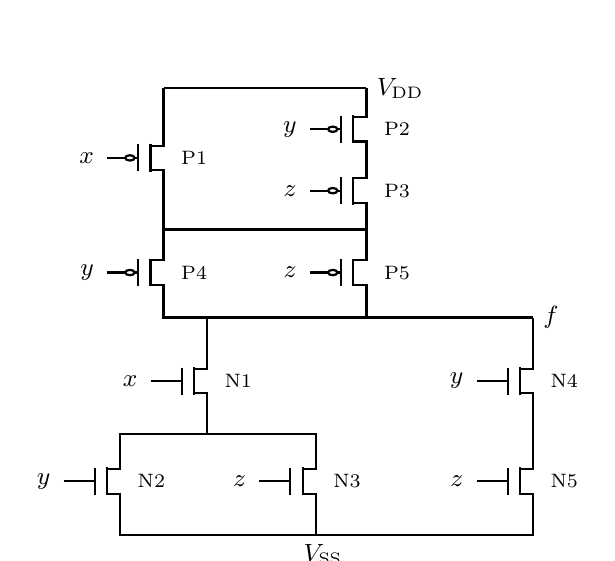
\begin{tikzpicture}[x=.92cm,y=.52cm,line width=.8pt,font=\small]
\MOS{P1}{-.6}{6.1}{x}{p}\MOS{P2}{2.2}{6.8}{y}{p}\MOS{P3}{2.2}{5.3}{z}{p}
\MOS{P4}{-.6}{3.3}{y}{p}\MOS{P5}{2.2}{3.3}{z}{p}
\draw (-.6,7.8)--(2.2,7.8) node[right] {$\VDD$};
\draw (-.6,7.8)--(P1t) (2.2,7.8)--(P2t) (P2b)--(P3t);
\draw (P1b)--(-.6,4.35)--(2.2,4.35)--(P3b);
\draw (-.6,4.35)--(P4t) (2.2,4.35)--(P5t);
\draw (P4b)--(-.6,2.2)--(4.5,2.2) node[right] {$f$};\draw (P5b)--(2.2,2.2);
\MOS{N1}{0}{.65}{x}{n}\MOS{N2}{-1.2}{-1.8}{y}{n}\MOS{N3}{1.5}{-1.8}{z}{n}
\MOS{N4}{4.5}{.65}{y}{n}\MOS{N5}{4.5}{-1.8}{z}{n}
\draw (0,2.2)--(N1t) (4.5,2.2)--(N4t);
\draw (N1b)--(0,-.65)--(-1.2,-.65)--(N2t);\draw (0,-.65)--(1.5,-.65)--(N3t);
\draw (N4b)--(N5t);
\draw (N2b)--(-1.2,-3.1)--(4.5,-3.1)--(N5b);\draw (N3b)--(1.5,-3.1);
\node[below] at (1.6,-3.1) {$\VSS$};
\end{tikzpicture}
\end{center}
\textbf{Gate labels in this diagram.} P4/N4 are controlled by $y$ and P5/N5 by $z$; repeated labels denote independent devices.
The dual PUN is $(p_x\parallel(p_y\hbox{ series }p_z))$ in series with $(p_y\parallel p_z)$. It uses true literals only and needs \textbf{10 transistors}.
\begin{center}\begin{tabular}{ccc|c}\toprule
$x$&$y$&$z$&$f$\\\midrule
0&0&0&1\\0&0&1&1\\0&1&0&1\\0&1&1&0\\
1&0&0&1\\1&0&1&0\\1&1&0&0\\1&1&1&0\\\bottomrule
\end{tabular}\end{center}
\textbf{Reference comparison.} The supplied answer implements the equivalent PDN $(x+y)(x+z)(y+z)=xy+xz+yz$, using six nMOS and six pMOS. Factoring the majority expression saves two transistors. All eight combinations pass the independent PDN/PUN complement check.
\end{document}
